% Section 7: Results (new in A3). Data and statistics only; interpretation is in Section 8.
\section{Results}\label{sec:results}
\emph{Execution.} All 930 Mac runs (93 cells $\times$ 10 forks), all 280 control runs, and all 318 Intel runs completed; every batch's idle pair agreed (Mac 0.009 to 0.020\,W, Intel 3.2 to 4.0\,W). Unless stated otherwise, values are medians over forks of raw energy per operation (J/op): CPU-cluster energy on the Mac and package energy on Intel. Mac CPU-bound fork-to-fork CV was below 1\%. Table~\ref{tab:hyp-results} summarizes the tests; per-cell statistics and all test results are in the replication package.

\begin{table}[tb]
\caption{Hypothesis decisions (Mac, Holm-corrected within families, $\alpha = 0.05$). Intel has 3 forks per cell and is descriptive (Section~\ref{sec:planning-analysis}). $\varepsilon^2$ and Cliff's~$\delta$ are the effect sizes.}
\label{tab:hyp-results}
\scriptsize
\setlength{\tabcolsep}{2.5pt}
\begin{tabular}{@{}lp{7.1cm}@{}}
\toprule
H0 & Mac result \\
\midrule
Main & Rejected on every workload ($\varepsilon^2$ = 0.92 CPU, 0.94 SLEEP, 0.85 SOCKET). \\
H0-1.1 & Rejected for FP, FJ, and VT on every workload (9 of 9; $\varepsilon^2$ 0.57 to 0.96). \\
H0-1.2 & Rejected on every workload: SEQ is not the lowest-energy option (split sample, $\delta = 1$). \\
H0-1.3 & Rejected: $\rho = 0.987$ between time/op and energy/op over the 23 CPU cells. \\
H0-2.1 & Rejected at every $p$ on every workload (21 of 21; $\varepsilon^2$ 0.64 to 0.92). \\
H0-2.2 & Rejected only on CPU at $p = 256$ ($\delta = -0.96$); on SLEEP and SOCKET $\mathrm{VT}_{256}$ is below PT, $\mathrm{FP}_{256}$, $\mathrm{FJ}_{256}$ ($\delta = -1$) but not below idle-subtracted SEQ. \\
H0-3.1 & Rejected in 14 of 24 cells: all 8 on CPU, 3 of 8 on SLEEP and on SOCKET. \\
H0-3.2 & Rejected on every workload at $p = 4$ and 16 ($\varepsilon^2$ 0.60 to 0.91). \\
\bottomrule
\end{tabular}
\end{table}

\subsection{RQ1: Concurrency Level, Sequential Execution, and Time}\label{sec:res-rq1}
Figure~\ref{fig:lambda} and Table~\ref{tab:cpu} show the CPU-bound results. On the Mac, every construct at $p = 1$ runs at about 1030\,ms and 4.05\,J/op, and energy/op falls monotonically with $p$ to 1.70\,J/op at $p \geq 16$, 2.4 times less than SEQ at 6.7 times the speed. At equal $p \geq 16$ the constructs lie within 3\% of each other; $\mathrm{VT}_{256}$ (1.704\,J/op) is the only configuration significantly lower than every alternative at its level (H0-2.2). On Intel, the lowest CPU energy/op (2.12 to 2.16\,J/op for VT, reused FP, and reused FJ at $p = 256$) is 4.0 times below SEQ (8.38\,J/op) at 12 times the speed.

Figure~\ref{fig:evt} plots energy/op against time/op. On the Mac the cells lie on one increasing curve (H0-1.3, $\rho = 0.987$). On Intel, $\rho = 0.45$ over the 15 unpinned CPU cells (Table~\ref{tab:cpu}): PT and the per-operation pools at $p = 256$ ran at the 25\,W package limit with E-core clocks of 2950 to 3222\,MHz (P cores up to 3725\,MHz) and were 28 to 33\% faster but used 28 to 38\% more energy than VT and the reused pools, whose E-core clocks were about 1700\,MHz; the three-fork ranges do not overlap. In the control experiment on the Mac, reusing the pool changed CPU energy/op by at most 2\% (reused FP 1.716, reused FJ 1.725, $\mathrm{VT}_{256}$ 1.721\,J/op).

On the blocking workloads (Figure~\ref{fig:lambda}, middle and right), the bounded pools follow the analytic floor $\lceil 256/p \rceil \times d$, and SEQ, which mostly sleeps, has raw energy/op 34 times that of $\mathrm{VT}_{256}$ on SLEEP but an idle-subtracted energy/op of about zero (0.004\,J/op, within the detection limit).

\begin{figure*}[tb]
\centering
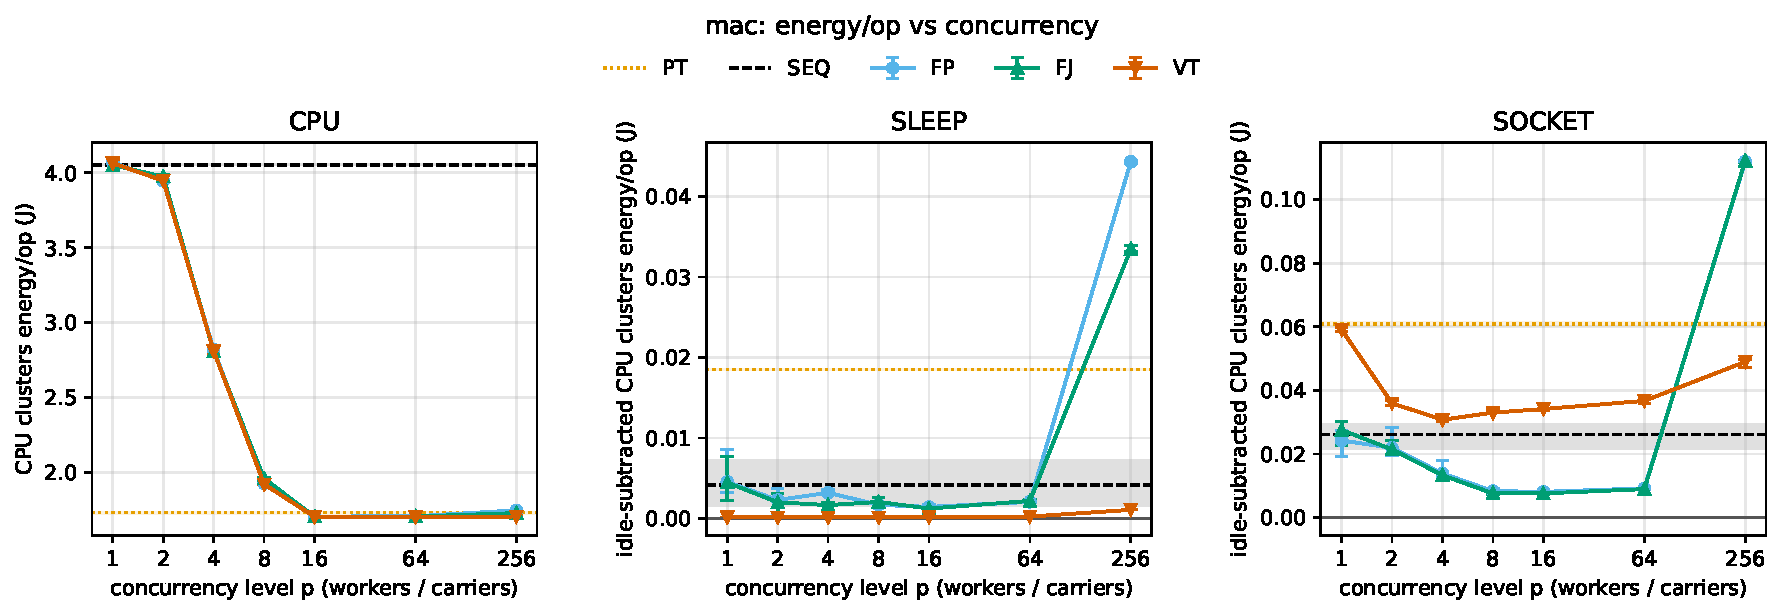
\includegraphics[width=0.78\textwidth]{figures/mac-lambda.pdf}
\caption{Mac energy/op against concurrency level $p$ (medians, IQR bars): raw CPU-cluster energy on CPU, idle-subtracted on SLEEP and SOCKET; PT and SEQ, which have no $p$, are horizontal lines; the grey band is SEQ's IQR.}
\label{fig:lambda}
\end{figure*}

\begin{table}[tb]
\caption{CPU-bound workload: medians of J/op and ms/op. Mac: CPU clusters, 10 forks (reused pools from the control run); Intel: package, unpinned, 3 forks.}
\label{tab:cpu}
\scriptsize
\setlength{\tabcolsep}{4pt}
\begin{tabular}{@{}lrrrrr@{}}
\toprule
 & \multicolumn{2}{c}{Mac M4} & \multicolumn{3}{c}{Intel 255H} \\
\cmidrule(lr){2-3}\cmidrule(l){4-6}
Configuration & J/op & ms/op & J/op & ms/op & W \\
\midrule
SEQ & 4.05 & 1029 & 8.38 & 1976 & 4.2 \\
PT & 1.73 & 156 & 2.72 & 109 & 25.0 \\
$\mathrm{FP}_4$ / $\mathrm{FJ}_4$ / $\mathrm{VT}_4$ & 2.80--2.82 & 292--294 & 3.70--3.74 & 510--557 & 6.7--7.2 \\
$\mathrm{FP}_{16}$ / $\mathrm{FJ}_{16}$ / $\mathrm{VT}_{16}$ & 1.70 & 154--155 & 2.14--2.29 & 162--174 & 13.1--13.7 \\
$\mathrm{FP}_{256}$, new each op & 1.75 & 160 & 2.92 & 117 & 25.0 \\
$\mathrm{FJ}_{256}$, new each op & 1.73 & 157 & 2.82 & 113 & 25.0 \\
$\mathrm{VT}_{256}$ & 1.70 & 154 & 2.12 & 162 & 13.1 \\
$\mathrm{FP}_{256}$, reused & 1.72 & 154 & 2.14 & 162 & 13.2 \\
$\mathrm{FJ}_{256}$, reused & 1.73 & 154 & 2.16 & 163 & 13.2 \\
\bottomrule
\end{tabular}
\end{table}

\begin{figure}[tb]
\centering
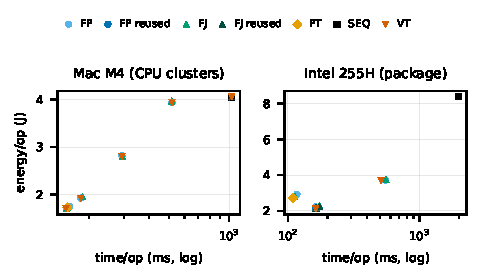
\includegraphics[width=0.9\columnwidth]{figures/cpu-energy-vs-time.pdf}
\caption{CPU-bound workload: cell-median energy/op against time/op. Mac: 23 cells of Experiment~1; Intel: 15 unpinned cells. The Intel points near 110\,ms are PT and the per-operation pools at $p = 256$.}
\label{fig:evt}
\end{figure}

\subsection{RQ2: Virtual Threads Against the Other Constructs}\label{sec:res-rq2}
Table~\ref{tab:blocking} gives the blocking workloads. \emph{Mac, Experiment~1.} At $p = 256$ on SLEEP, VT used 15 to 36 times less energy/op than PT, FJ, and FP at 14.4 against 20 to 23\,ms, and 0.0003 to 0.0004\,J/op with 1 to 64 carriers; the memory-subsystem family gave the same order (VT 0.0008, PT 0.0034, $\mathrm{FP}_{256}$ 0.011\,J/op). On SOCKET at $p = 256$, VT used 20\% less than PT and 56\% less than FP and FJ; its minimum was 0.031\,J/op with 4 carriers. Bounded pools with 8 to 64 workers used 0.0097 to 0.013\,J/op on SOCKET but took 57 to 421\,ms.

\emph{Control: reused pools.} At $p = 256$ on the Mac, reusing the pool lowered SLEEP energy/op from 0.045 to 0.0011\,J/op (FP) and from 0.034 to 0.0024\,J/op (FJ), against 0.0013\,J/op for $\mathrm{VT}_{256}$ in the same campaign: 0.86 and 1.80 times VT. On SOCKET, reused FP and FJ used 0.031 and 0.038\,J/op against 0.049\,J/op for VT (0.64 and 0.78 times) and were 5 to 8\% faster (19.1 and 19.6 against 20.6\,ms; all ten forks separate, Mann-Whitney $p = 0.0002$). On Intel, reused pools at $p = 256$ used 0.079 to 0.089\,J/op on SLEEP and 0.136 to 0.146\,J/op on SOCKET, 2.6 to 4.1 times less than the pools created per operation, and VT with 4 carriers used 0.038 (SLEEP) and 0.106\,J/op (SOCKET), the lowest values of each workload, with fork ranges that do not overlap those of the reused pools. $\mathrm{VT}_{256}$ on Intel drew 11 to 13\,W against 5 to 7\,W for the reused pools.

\emph{MIXED.} The last columns of Table~\ref{tab:blocking} show the control's compute-then-wait workload. On both platforms the constructs lie within 11\% (Mac) and 13\% (Intel) of each other in energy/op, and VT is the fastest configuration (Mac 49.2 to 49.6\,ms against 53.0\,ms or more; Intel 28.8\,ms against 29.7\,ms or more).

\begin{table*}[tb]
\caption{Blocking and MIXED workloads (MIXED: 1.5\,ms of computation, then a 10\,ms sleep per task): medians of raw J/op and ms/op. Mac: CPU clusters, 10 forks (reused pools from the control run, whose $\mathrm{VT}_{256}$ reference is 0.0013\,J/op on SLEEP and 0.049 on SOCKET); Intel: package (including about 3.3\,W idle), unpinned, 3 forks.}
\label{tab:blocking}
\scriptsize
\setlength{\tabcolsep}{4pt}
\begin{tabular}{@{}lrrrrrrrrrrrr@{}}
\toprule
 & \multicolumn{4}{c}{SLEEP} & \multicolumn{4}{c}{SOCKET} & \multicolumn{4}{c}{MIXED} \\
\cmidrule(lr){2-5}\cmidrule(lr){6-9}\cmidrule(l){10-13}
 & \multicolumn{2}{c}{Mac M4} & \multicolumn{2}{c}{Intel 255H} & \multicolumn{2}{c}{Mac M4} & \multicolumn{2}{c}{Intel 255H} & \multicolumn{2}{c}{Mac M4} & \multicolumn{2}{c}{Intel 255H} \\
\cmidrule(lr){2-3}\cmidrule(lr){4-5}\cmidrule(lr){6-7}\cmidrule(lr){8-9}\cmidrule(lr){10-11}\cmidrule(l){12-13}
Configuration & J/op & ms/op & J/op & ms/op & J/op & ms/op & J/op & ms/op & J/op & ms/op & J/op & ms/op \\
\midrule
SEQ & 0.0413 & 3728 & 9.33 & 2602 & 0.0600 & 3119 & 9.53 & 2640 & -- & -- & -- & -- \\
PT & 0.0187 & 21.3 & 0.201 & 31.6 & 0.0611 & 18.5 & 0.289 & 38.2 & 0.464 & 54.8 & 1.314 & 39.0 \\
$\mathrm{FP}_{16}$, new each op & 0.0040 & 232 & 0.592 & 165 & 0.0103 & 210 & 0.733 & 177 & -- & -- & -- & -- \\
$\mathrm{FP}_{256}$, new each op & 0.0445 & 20.0 & 0.281 & 42.9 & 0.1122 & 21.2 & 0.360 & 48.9 & 0.489 & 58.1 & 1.282 & 52.9 \\
$\mathrm{FJ}_{256}$, new each op & 0.0337 & 23.5 & 0.326 & 50.4 & 0.1124 & 20.6 & 0.411 & 60.3 & 0.479 & 56.8 & 1.218 & 54.8 \\
$\mathrm{FP}_{256}$, reused & 0.0011 & 18.0 & 0.089 & 18.5 & 0.0312 & 19.1 & 0.136 & 21.4 & 0.441 & 53.0 & 1.221 & 31.1 \\
$\mathrm{FJ}_{256}$, reused & 0.0024 & 19.6 & 0.079 & 13.0 & 0.0377 & 19.6 & 0.146 & 21.2 & 0.452 & 53.2 & 1.254 & 29.7 \\
$\mathrm{VT}_{256}$ & 0.0012 & 14.4 & 0.208 & 15.4 & 0.0492 & 20.6 & 0.242 & 21.3 & 0.451 & 49.6 & 1.241 & 30.4 \\
$\mathrm{VT}_4$ & 0.0003 & 14.8 & 0.038 & 10.7 & 0.0310 & 19.9 & 0.106 & 18.6 & -- & -- & -- & -- \\
$\mathrm{VT}_{16}$ & -- & -- & -- & -- & -- & -- & -- & -- & 0.441 & 49.2 & 1.158 & 28.8 \\
\bottomrule
\end{tabular}
\end{table*}


\subsection{RQ3: Restriction to Efficiency Cores}\label{sec:res-rq3}
\emph{Mac, BACKGROUND against DEFAULT QoS} (Table~\ref{tab:rq3}). CPU work became 4.2 to 5.5 times slower and used 8 to 15 times less energy/op; on SLEEP a 10\,ms sleep lasted 177\,ms (AX5). Under BACKGROUND on SLEEP, PT used 0.0074\,J/op and VT 0.0022 to 0.0023\,J/op at $p \in \{4, 16\}$, against 0.0187 and 0.0003\,J/op under DEFAULT. \emph{Cluster split} (H0-3.2). Under DEFAULT QoS, the E-cluster share of CPU energy was 13 to 16\% for PT on every workload, 99 to 100\% for VT, FP, and FJ on SLEEP, 29 to 30\% for VT and 86 to 100\% for FP and FJ on SOCKET, and 0.2 to 0.3\% at $p = 4$ and 13\% at $p = 16$ on CPU.

\emph{Intel, equal-count pinning} (two cores of one class, $p = 4$; Table~\ref{tab:rq3}). On SLEEP, PT drew 12.5\,W on 2P and 7.8\,W on 2E at 15.5 and 16.5\,ms, and used 5.2 (2P), 3.5 (2E), and 6.9 (2LP-E) times the energy/op of $\mathrm{VT}_4$, which took 10.7 to 11.1\,ms on every class; on SOCKET the ratios were 3.0, 2.4, and 3.7. On CPU, 2E took 1273 to 1296\,ms against 1017 to 1041 on 2P, and 2LP-E 1485 to 1908\,ms.

\begin{table}[tb]
\caption{Restriction to efficiency cores. Top: Mac, BACKGROUND over DEFAULT QoS (ratios of medians, $p \in \{4, 16\}$, all constructs). Bottom: Intel pinned to two cores, medians of J/op (CPU: range over PT, FP, FJ, VT, and reused FP).}
\label{tab:rq3}
\scriptsize
\setlength{\tabcolsep}{3pt}
\begin{tabular}{@{}lrrrrr@{}}
\toprule
\multicolumn{6}{@{}l}{\emph{Mac M4: BACKGROUND / DEFAULT}} \\
 & \multicolumn{2}{c}{Time} & \multicolumn{3}{c}{Energy/op} \\
\midrule
CPU & \multicolumn{2}{c}{4.2--5.5$\times$} & \multicolumn{3}{c}{0.07--0.13$\times$} \\
SLEEP & \multicolumn{2}{c}{10--12$\times$} & \multicolumn{3}{c}{7--11$\times$ (PT 0.39$\times$)} \\
SOCKET & \multicolumn{2}{c}{1.0--1.8$\times$} & \multicolumn{3}{c}{0.69--1.62$\times$} \\
\midrule
\multicolumn{6}{@{}l}{\emph{Intel 255H: pinned, J/op}} \\
Arm & CPU & SLEEP PT & SLEEP $\mathrm{VT}_4$ & SOCKET PT & SOCKET $\mathrm{VT}_4$ \\
\midrule
2P & 5.39--5.53 & 0.195 & 0.037 & 0.297 & 0.099 \\
2E & 5.12--5.33 & 0.129 & 0.037 & 0.210 & 0.088 \\
2LP-E & 8.26--9.18 & 0.264 & 0.038 & 0.628 & 0.172 \\
\bottomrule
\end{tabular}
\end{table}
